% \begin{frame}
% 	\frametitle{Wirkungsquerschnitt}
% 	\begin{figure}
% 	\begin{center}
% 	  \includegraphics[width=0.3\textwidth]{../img/atlas_higgs_event.png}
% 	  \caption{Produkte einer Proton-Proton-Kollision beim ATLAS-Experiment am CERN (Quelle: https://cds.cern.ch/record/1459496)}
% 	\end{center}
% 	\end{figure}
% 	\begin{itemize}
% 		\item Bei Streuprozessen ist der Endzustand nicht eindeutig bestimmt
% 		\item Der Wahrscheinlichkeit eines bestimmten Endzustandes wird durch den Wirkungsquerschnitt $\sigma$ beschrieben.
% 		\item Differentieller Wirkungsquerschnitt $\frac{\difd \sigma}{\difd O}$ in Bezug auf \\
% 			  Observable $O$ (z.B. Raumwinkel $\Omega$, Transversalimpuls $p_\text{T}, \ldots$)
% 	\end{itemize}
% \end{frame}

\section{Theoretische Grundlagen}

\subsection{Das Standardmodell}
 \begin{frame}
 	\frametitle{Das Standardmodell}
 	\begin{figure}
 	\begin{center}
 	  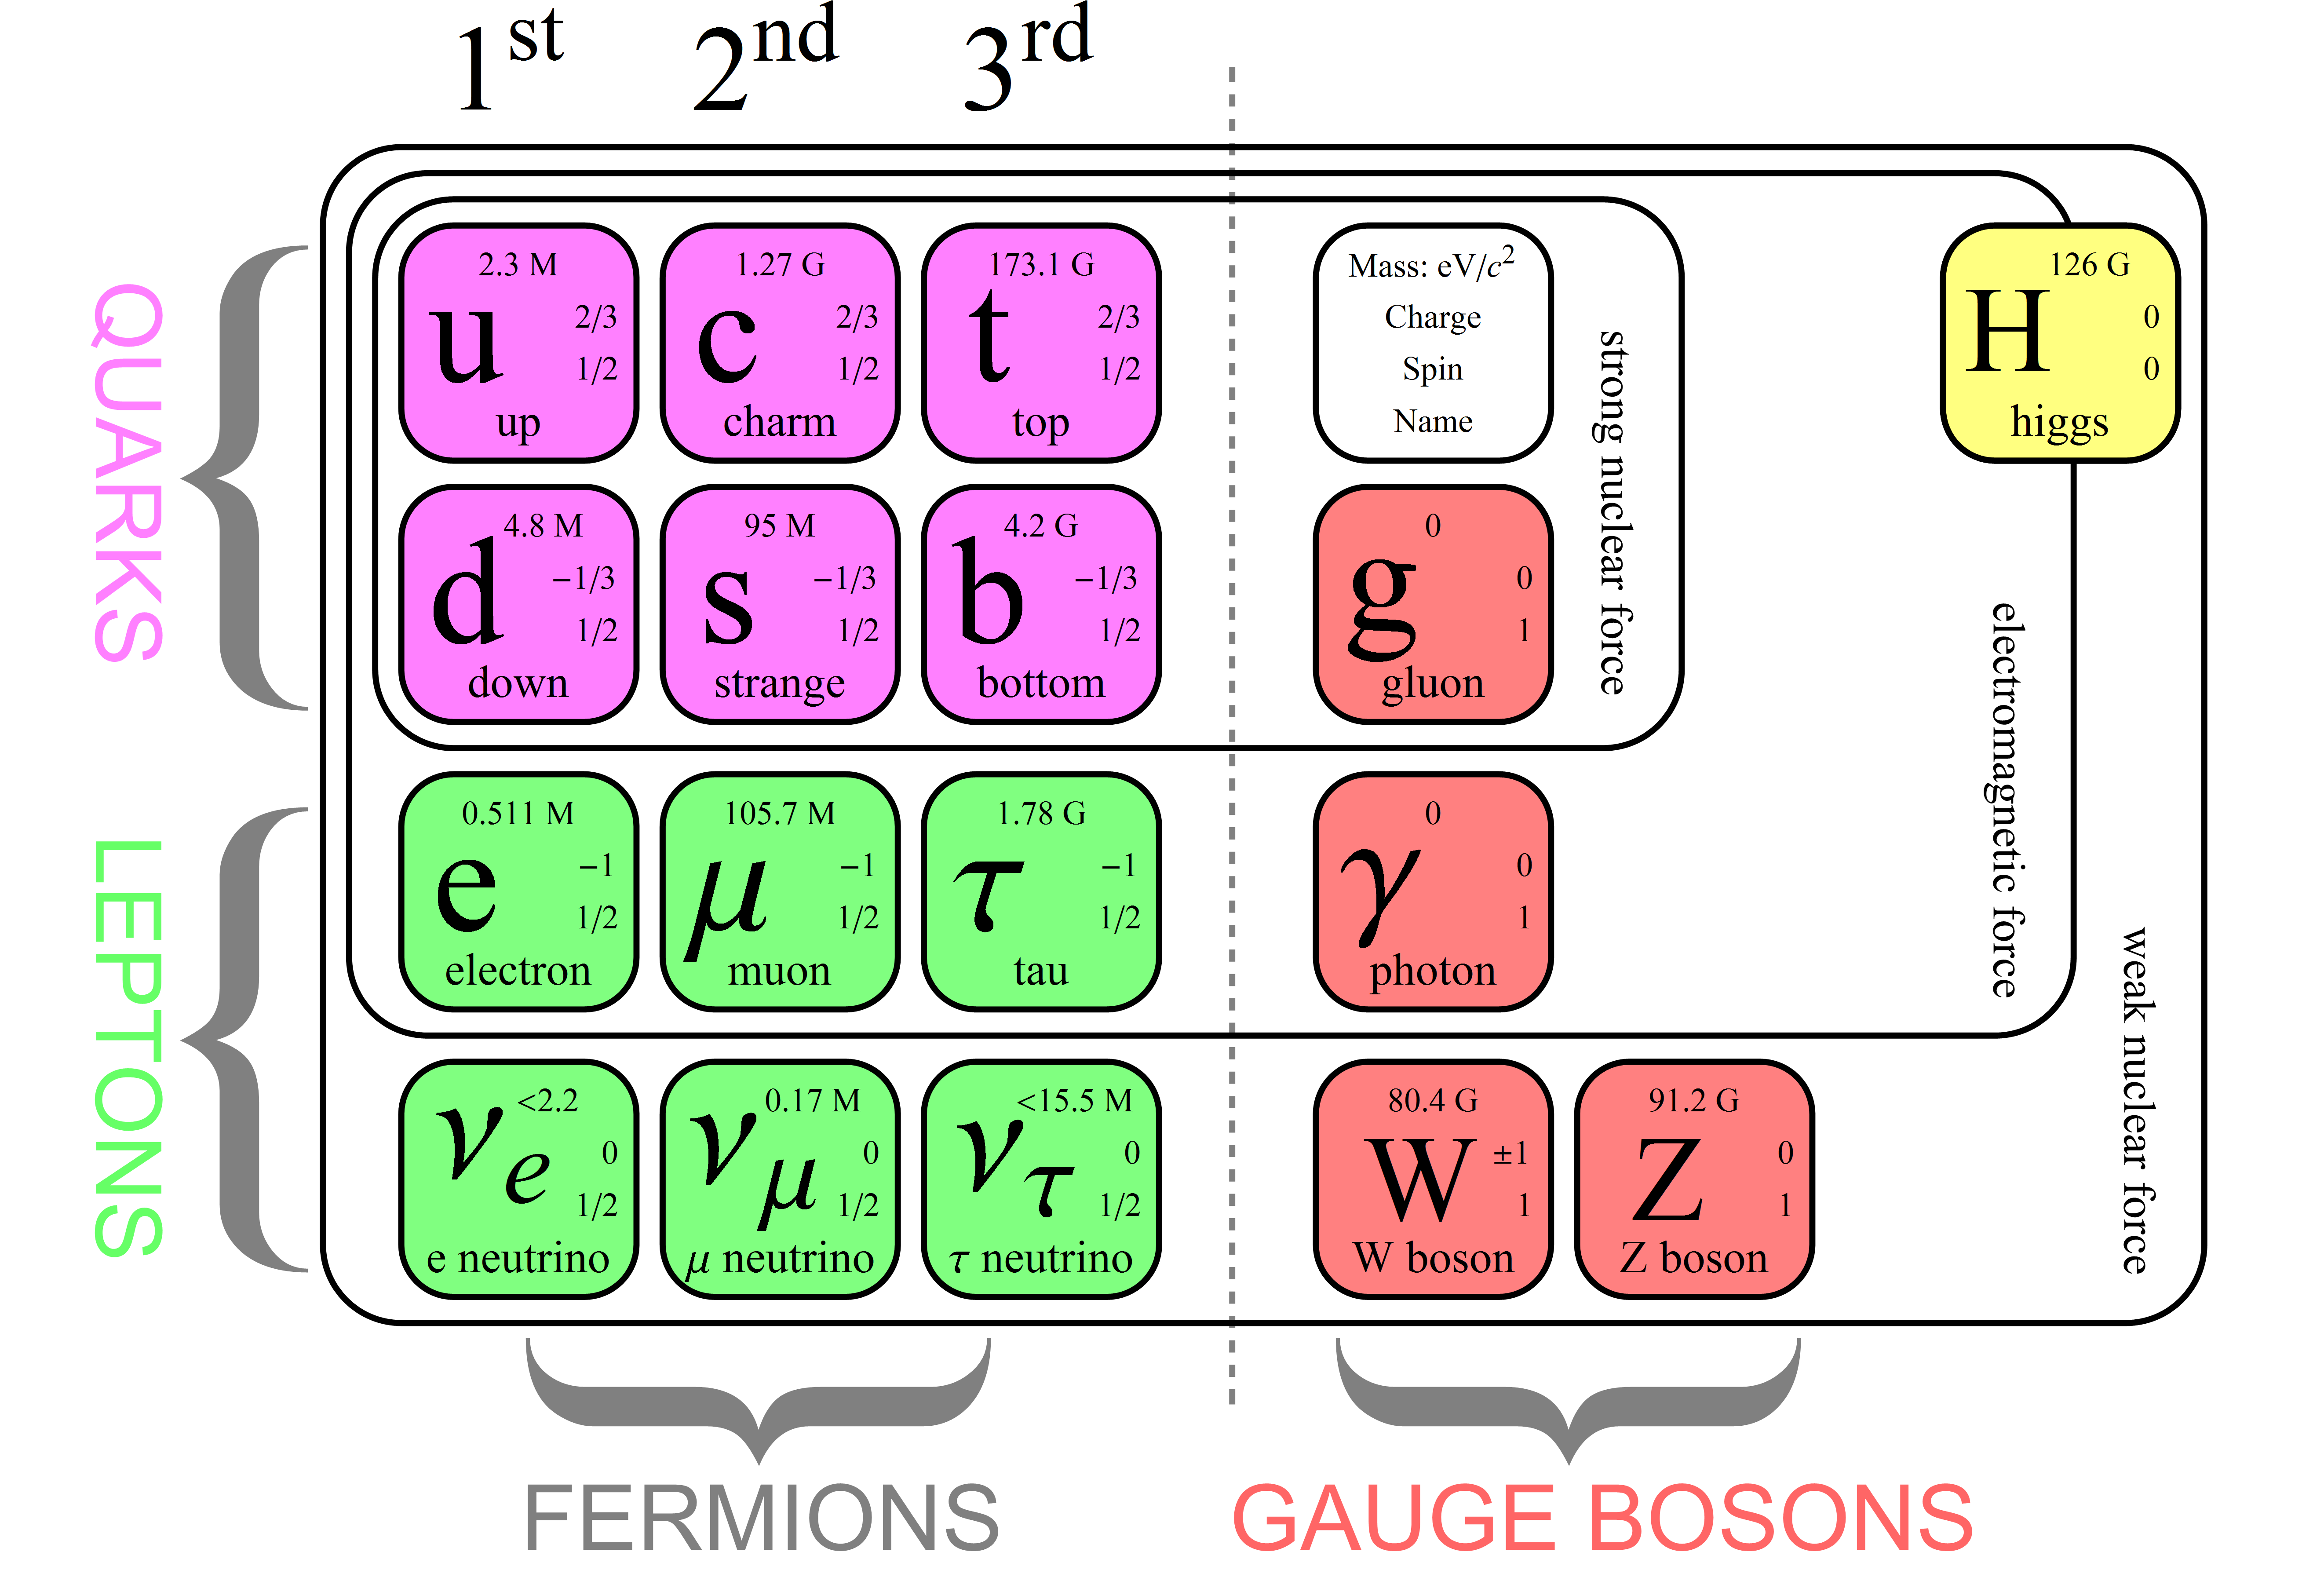
\includegraphics[width=0.9\textwidth]{graphics/SM1.png}
 	\end{center}
	\end{figure}
 \end{frame}
\subsection{Elektroschwache Wechselwirkung}
\begin{frame}
	\frametitle{Weinbergwinkel und Kopplungsstärken}
	\begin{center}
		\begin{equation*}
			\ket{\gamma} =  cos(\theta_w)\ket{B^0} + sin(\theta_w) \ket{W^0}
		\end{equation*}
		\begin{equation*}
		\ket{Z^0} = -sin(\theta_w) \ket{B^0} + cos(\theta_w) \ket{W^0}
		\end{equation*}\\
		\begin{equation*}
		\textcolor{lightgray}{g_V^f = I^f_3-2 Q_f sin^2(\theta_w)}
		\end{equation*}
		\begin{equation*}
		\textcolor{lightgray}{g_A^f = I^f_3}
		\end{equation*}
	\end{center}
\end{frame}
\begin{frame}
	\frametitle{Weinbergwinkel und Kopplungsstärken}
	\begin{center}
		\begin{equation*}
		\textcolor{lightgray}{\ket{\gamma} =  cos(\theta_w)\ket{B^0} + sin(\theta_w) \ket{W^0}}
		\end{equation*}
		\begin{equation*}
		\textcolor{lightgray}{\ket{Z^0} = -sin(\theta_w) \ket{B^0} + cos(\theta_w) \ket{W^0}}
		\end{equation*}
		\\
		\begin{equation*}
			g_V^f = I^f_3-2 Q_f sin^2(\theta_w)
		\end{equation*}
		\begin{equation*}
			g_A^f = I^f_3
		\end{equation*}
	\end{center}
\end{frame}

\subsection{$e^+e^-$ Kollisionen}
\begin{frame}
	\frametitle{$e^+e^- \rightarrow f\bar{f}$ }
	\begin{center}
		\begin{figure}
			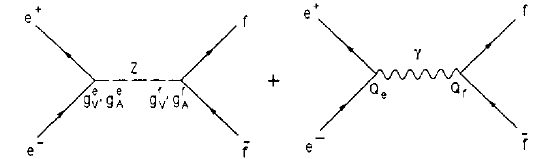
\includegraphics[width=0.8\textwidth]{graphics/annihilation.png}
		\end{figure}
	\end{center}
\end{frame}
\begin{frame}
	\frametitle{Der Wirkungsquerschnitt}
	\begin{center}
		\begin{equation*}
		\sigma_f(s) = \frac{12\pi}{M_Z^2} \frac{s\Gamma_e\Gamma_f}{(s-M_Z^2)^2+s^2\Gamma_Z^2/M_Z^2}
		\end{equation*}
		
	\end{center}
\end{frame}
\begin{frame}
	\frametitle{Bhabha Streuung }
	\begin{center}
		\begin{figure}
			\includegraphics[width=0.8\textwidth]{graphics/Bhabbastreuung.png}
		\end{figure}
	\end{center}
	\begin{equation*}
	\frac{d\sigma_s}{d\Omega} \propto (1+cos^2(\theta)),\qquad\frac{d\sigma_t}{d\Omega}t \propto (1-cos(\theta))^{-2}
	\end{equation*}
\end{frame}
\subsection{Strahlungskorrekturen}
\begin{frame}
	\frametitle{Strahlungskorrekturen}
	\begin{figure}
		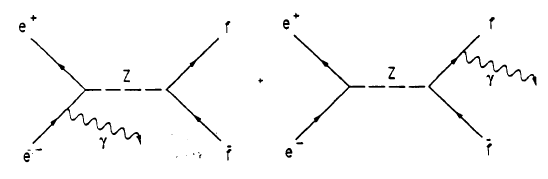
\includegraphics[width=0.75\linewidth]{graphics/Bremsstrahlungskorrektur}
	\end{figure}
	\begin{center}
	\begin{minipage}{0.4\linewidth}
			\begin{figure}
				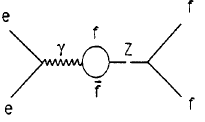
\includegraphics[width=0.8\linewidth]{graphics/presentationvertexschleifen}
			\end{figure}
	\end{minipage}
	\begin{minipage}{0.4\linewidth}
	\begin{figure}
			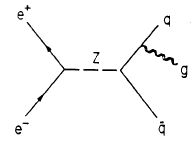
\includegraphics[width=0.8\linewidth]{graphics/presentation_QCDkorrektur}
	\end{figure}
	\end{minipage}
	\end{center}
\end{frame}

\subsection{Wirkungsquerschnitt und Zerfallsbreite}
\begin{frame}
	\frametitle{Wirkungsquerschnitt}
	\hspace{1cm} Ereignisrate bei Luminosität $L$:
	\begin{equation*}
	\scalebox{1.5}{$\dot{N} = \sigma \cdot L$}
	\end{equation*}
	\hspace{1cm} Wirkungsquerschnitt messen:
	\begin{equation*}
	\scalebox{1.5}{$\sigma = \frac{N}{\int L~\text{d}t}$}
	\end{equation*}
\end{frame}
\subsection{Vorwärts Rückwärts Asymmetrie}
\begin{frame}
	\frametitle{Vorwärts Rückwärts Asymmetrie}
	\begin{center}
		\begin{equation*}
		\sigma_f=\int_{0}^{1}\frac{\text{d}\sigma}{\text{d}cos(\theta)}~\text{d}cos(\theta)
		\end{equation*}
		\begin{equation*}
		\sigma_b=\int_{-1}^{0}\frac{\text{d}\sigma}{\text{d}cos(\theta)}~\text{d}cos(\theta)
		\end{equation*}
		\\
		\begin{equation*}
		\textcolor{lightgray}{A_{fb}=\frac{\sigma_f-\sigma_b}{\sigma_f+\sigma_b}}
		\end{equation*}
	\end{center}
\end{frame}
\begin{frame}
	\frametitle{Vorwärts Rückwärts Asymmetrie}
	\begin{center}
		\begin{equation*}
		\textcolor{lightgray}{\sigma_f=\int_{0}^{1}\frac{\text{d}\sigma}{\text{d}cos(\theta)}~\text{d}cos(\theta)}
		\end{equation*}
		\begin{equation*}
		\textcolor{lightgray}{\sigma_b=\int_{-1}^{0}\frac{\text{d}\sigma}{\text{d}cos(\theta)}~\text{d}cos(\theta)}
		\end{equation*}
		\\
		\begin{equation*}
		A_{fb}=\frac{\sigma_f-\sigma_b}{\sigma_f+\sigma_b}
		\end{equation*}
	\end{center}
\end{frame}
\begin{frame}
	\frametitle{Vorwärts Rückwärts Asymmetrie}
	\begin{center}
		Für Leptonen am Resonanzpeak:
		\begin{equation*}
		A_{fb}^{\ell,peak}\approx 3 \left ( \frac{g^{\ell}_V}{g^{\ell}_A} \right )^2=3\cdot (1-4 sin^2(\theta_w))
		\end{equation*}
	\end{center}
\end{frame}